\documentclass{acm_proc_article-sp}

\usepackage{amsmath}
\usepackage{verbatim}
\usepackage{textcomp}
\usepackage{graphicx}
\usepackage{subcaption}
\usepackage{url}
\usepackage{multicol}
\usepackage{tikz}
\usetikzlibrary{positioning}
\usepackage{wasysym}


\begin{document}

\title{Montreal Real Estate Pricing \\
{\normalsize Code available at: \url{https://github.com/mike-n-7/ML4}}} 
\subtitle{}

\numberofauthors{2} 
\author{
% 1st. author
\alignauthor 
Michael Noseworthy \\
	\affaddr{260512169}
% 2nd. author
\alignauthor Benjamin La Schiazza\\
	\affaddr{260531181}
}

\date{Dec3}

\maketitle
\begin{abstract}

\end{abstract}

\section{Introduction}

	The real estate market is one of the most important markets in the modern economy because of the nature of the goods exchanged. Shelter is a fundamental need for humans and therefore there is a collective interest in pricing homes correctly. While there are other factors in play, an ill-informed party on either side of the transaction can be burned for non-trivial sums. Any insight into pricing homes properly and consistently would be of great interest to all parties involved. 
	
	There have been a number of attempts to model real estate prices using Machine Learning approaches. One of the efforts that was of interest involved pricing Boston suburban homes. [1] The results from this study were very impressive and influenced our choice of features for our data. In this paper, they explored the use of a Linear SVM regression and a partial least squares regression. The former yielded a means-squared error (MSE) of \$10,000 while the latter had a MSE of \$25,000. The interesting point however from their paper is their feature set which included distance to radial highways, density of non-retail businesses in the area as well as local crime rate. These results assured us that decent results have been achieved with the above model of real estate in a comparable city and serve as a benchmark for the results that follow. 
	
	The goal of this project was to attempt to model Montreal homes in its various boroughs while using open-data from the city of Montreal. [2] Not wanting to simply repeat results that have been obtained before, and ultimately constrained by the data sets at our disposal, we opted to explore the use of different characteristics in describing and modelling homes in the city. We hope to investigate the role of other municipal infrastructure in determining the value of homes and in doing so, convince policy makers that the collection, aggregation and dissemination of municipal/city data can be beneficial to its residents.


\section{Problem Definition and Description of data}
	
	This project aims to model Montreal housing prices based on a specific set of features in order to determine their importance in marketing a home. As there are all sorts of real estate available on the market, we focused on homes and condos. As alluded to above, we wanted to explore the role that municipal infrastructure has on the prices of homes, something that hasn't been explored in much depth. It is hence a regression task to determine the price of a property.
	
	Our data samples consist of standard descriptions of each property as well as the number of various municipal establishments within 3 kilometers of the property. This radius was chosen because it represents what we feel is a comfortable walking distance whether it is within the heart of the city or in a suburb. The learning algorithms used include traditional Linear Regression, Lasso Regression and K-nearest neighbours (which seemed appropriate!). 

\subsection{Data}

	The real estate market, unlike other traditional markets, does not have a centralized trading "floor" or venue. Parties have the option to deal with an agent or sell the house on their own. As a result price information on available properties isn't centralized. All of the housing data had to be retrieved from brokerage web sites. DuProprio and Royal Lepage web sites were used to get the data needed. They did not offer convenient API's so the sites had to be scraped for the necessary data. While this provided all the standard descriptors of properties, datasets released by the city of Montreal were needed to locate police stations, family-friendly buildings, handicap friendly buildings as well as numerous other notable infrastructure. Coordinate information for both properties and these entities were used to count instances within a walking radius.
	
	In all, 9717 data points were collected. Data points with abnormally high prices (defined in our case as >\$750000) were removed as there were very few training example in this regime which could adversely affect our ability to generalize. As alluded to, the main features were property descriptors (eg. type of property, living area, neighbourhood, latitude, longtitude, number of bathrooms, number of bedrooms) and counts of local municipal infrastructure (eg. fire stations, police stations, monuments, emergency shelters, family quality buildings...). There were [COUNT] features in all and the full list can be found with our code base.
	
\subsection{Missing Data}

	Because our dataset was scraped off of websites, there were a lot of data that were missing. These websites do not hold strict standards as to which features must be included in a house listing and which features may be excluded. Thus not every listing will include all the features we want to include in our model. Figure \ref{fig:missingdata} shows the number of entries that were missing each feature. Note only features with missing data are shown in this figure. Intuitively, these features will have an impact on predicting house price; for example a house with greater living area can be expected to cost more than a similar house that has less living area. 
	
	The algorithms we chose to apply are not ammenable to missing data. Both linear regression and k-nearest neighbours expect to see a value for each feature. Naively replacing this missing data with a value of zero or an innappropriate value can have an adverse effect by creating outliers in the data and generating more noise. We do not wish to remove features that include missing data as this will hurt the richness of our dataset and be detrimental to our predictive ability.
	
	We decided to look at 3 approaches to dealing with missing data: removing instances with missing data altogether, predicting missing data using Expectation Maximum [3] and predicting missing data with the mean of the features. 
	
	\begin{figure}[h!]
   		\centering
  		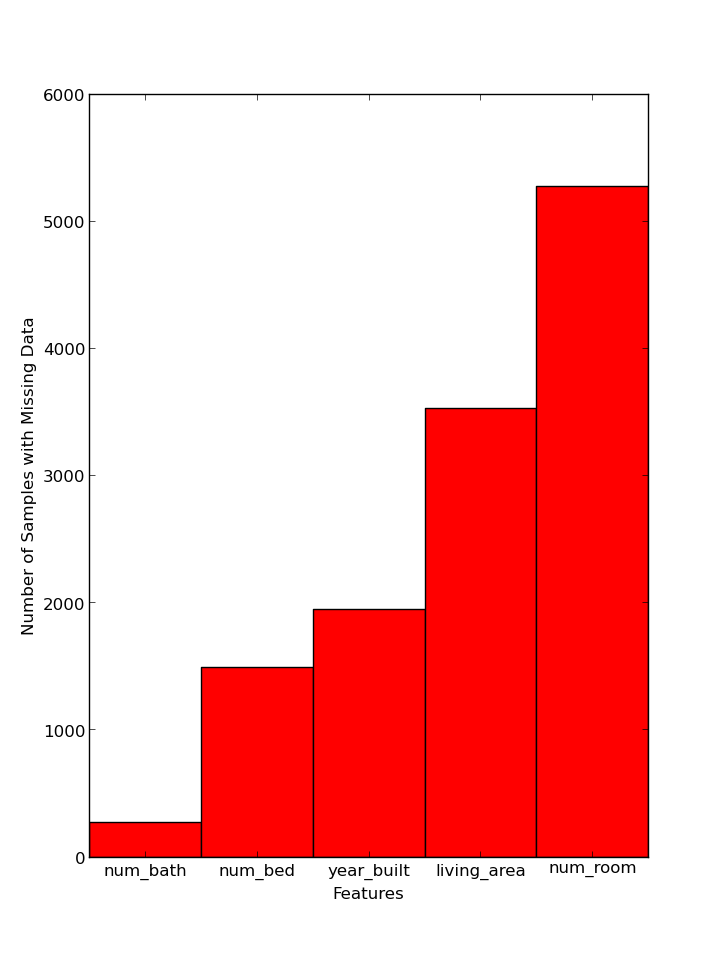
\includegraphics[width=\linewidth]{missing_data.png}
    		\caption{Number of instances with the above features missing. }
    		\label{fig:missingdata}
	\end{figure}
	
	By removing instances that included missing data, we reduced our dataset size to 2289 entries. This dramatic decrease is worrisome as we are losing more than half our data. Thus we also investigate how we can estimate the values of the missing data.

	The simplest method of imputing missing data is by taking the mean of each feature from the instances that are not missing that feature. Then we replace eash missing observation with its respective mean. Although this method allows us to keep all of our data, we are effectively adding bias to the data which may be detrimental to our predictive power.
	
	Finally, we try to estimate missing values by using an expectation-maximization like approach. We start by giving each missing value a default value, say its feature's mean. Then we repeatedly try to train a probabilistic model and estimate the values of the missing data until the values converge. In our implementation of this method, we use the scikit-learn MultinomialNB model to estimate missing data. For each feature that has missing data, a model is built using the other features trying to predict the missing feature. Then we use that model to re-estimate the missing data. Note the main limitations from this model arise from the assumptions of the Naive Bayes algorithm. For this method to be effective, the conditional independence assumption must hold and the other features must to rich enough to predict the features with missing data.
	
\section{Methodology}
	
	Due to the fact that there was a significant amount of missing data, we investigated not only algorithm performance but also methods for treating the missing data. Each algorithm was run on the three datasets resulting from these treatments. Algorithms were optimized for better results on training sets and a held out test set was used for final evaluation.
	
\subsection{Features}
	
	Features consisted of two broad categories, property descriptors and integer counts of the number of instances of municipal infrastructure within walking distance from the datapoint. Many of the features were inherently numerical so they remained untouched. Categorical data such as the property type (house, condo etc...) or the year it was sold (2002-unsold) could have been encoded using integer codes. Research has shown however that one-hot encoding yields better results. [4] These two characteristics hence exploded into a set of binary features.
	
\subsection{Algorithm Selection}
	Below is a brief description of the algorithms considered.
	
\subsubsection{Linear Regression}
\subsubsection{Lasso Regression}
\subsubsection{K Nearest Neighbours}

\subsection{Implementation Details}
	Raw data had to be scraped from real estate websites. To do so we used the popular Scrapy framework available for python [6]. A spider was written for each website and data from which was loaded through a script into a cohesive raw dataset. This raw data was then cleansed by removing outliers and bad data and extended using the Montreal datasets as discussed previously. All scripts for collecting and pre-processing of data is available in the code base (though Scrapy will need to be installed in order to scrape raw data).
	
	All the algorithms used were implemented in the scikit-learn library. [5] It provides efficient implementations of many useful algorithms and procedures and therefore we wanted to take advantage of the fact that it is available for use. Beyond the implementations of the regression algorithms, it was also used to set up our K sets for our K-Fold cross-validation procedure. 

\subsection{Training/Testing}


\section{Results}
	 The results were generally a bit disappointing when compared to the benchmark paper referenced in the Introduction [1]. Analysis however offers many plausible reasons for this as well as interesting insights. 
	 
\subsection{Linear Regression}
	Below compares the performance of Linear Regression over the three datasets representing approaches to handling missing data. Best performance was with the malformed data removed and yielded a MSE of about \$45,000.
	 
	 \begin{figure}[H]
   		\centering
  		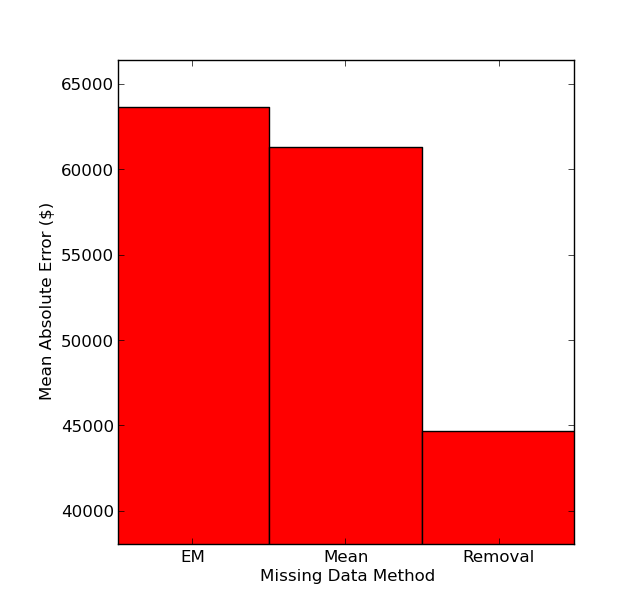
\includegraphics[width=\linewidth]{linear_regression_tuning.png}
    		\caption{Performance of Linear Regression algorithm}
    		\label{fig:linreg}
	\end{figure}
	
\subsection{Lasso Regression}
	Lasso's lambda parameter was optimized but performance seemed to be only marginally affected. Figure 3 shows once again that removing the missing data was most fruitful. Best MSE was approximately \$44,000.
	
	 \begin{figure}[H]
   		\centering
  		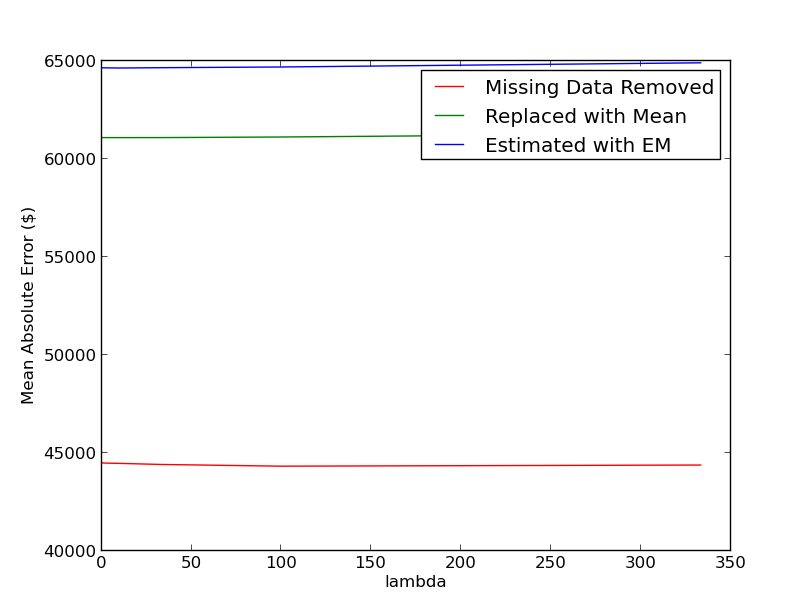
\includegraphics[width=\linewidth]{lasso_tuning_plot.png}
    		\caption{Performance of Lasso Regression algorithm}
    		\label{fig:lassoreg}
	\end{figure}
	
\subsection{K Nearest Neighbours}
	The optimal K was [INSERT], as shown below. Once again simply removing the bad data yielded the best results. 
	
	\begin{figure}[H]
   		\centering
  		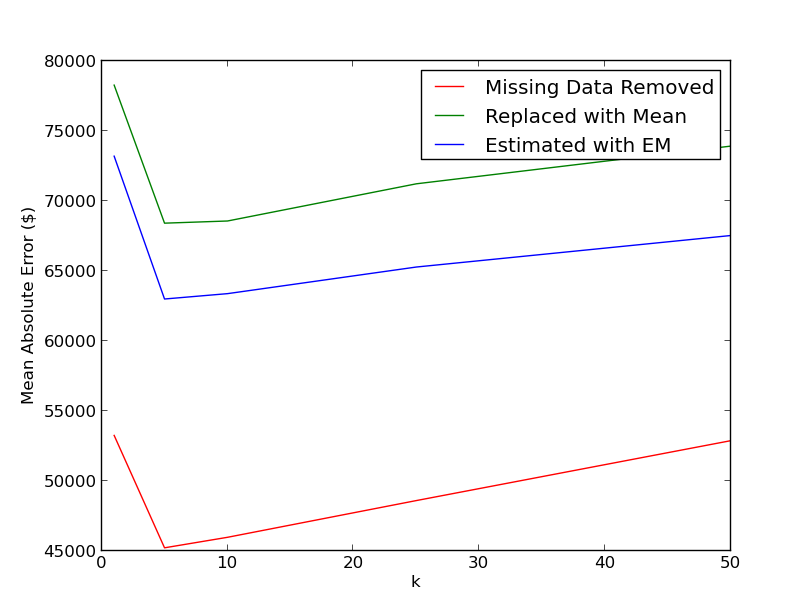
\includegraphics[width=\linewidth]{knn_tuning.png}
    		\caption{Performance of K-Nearest Neighbours as a function of K}
    		\label{fig:knn}
	\end{figure}


\section{Discussion}

\end{document}
